\chapter{Verifica}\label{chp:verifica}
In fase di verifica si è fatto uso della funzione \texttt{print\_update(\dots)} per monitorare l'avanzamento della simulazione \textit{step-by-step}, con l'obiettivo di controllare che l'evoluzione dello stato del sistema avvenisse fedelmente ai modelli precedentemente descritti (capp. \ref{chp:modello-concettuale}, \ref{chp:modello-specifiche}, \ref{chp:modello-computazionale}).

\begin{figure}[ht]
\centering
\begin{subfigure}[b]{0.475\textwidth}
\centering
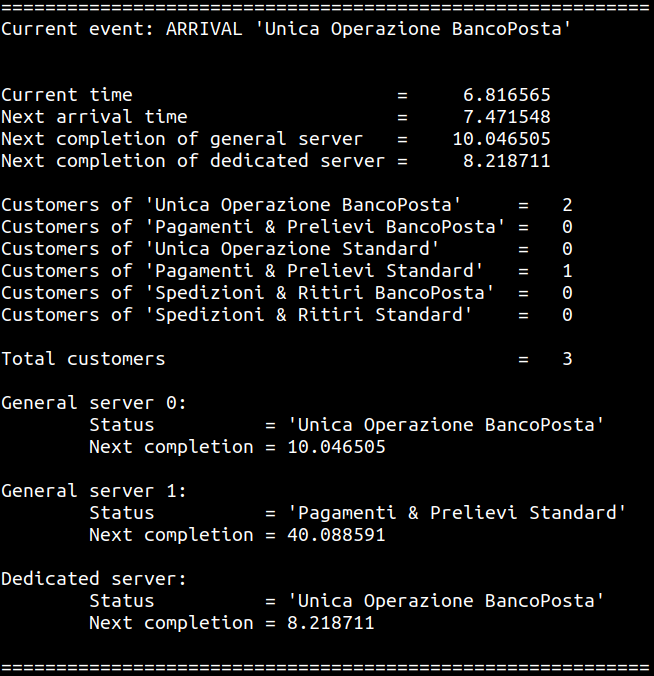
\includegraphics[width=\textwidth]{screenshots/original/ded_server_changes_behaviour}
\caption{Cambio del comportamento del server dedicato}    
\label{fig:verifica-1a}
\end{subfigure}
\hfill    
\begin{subfigure}[b]{0.475\textwidth}  
\centering 
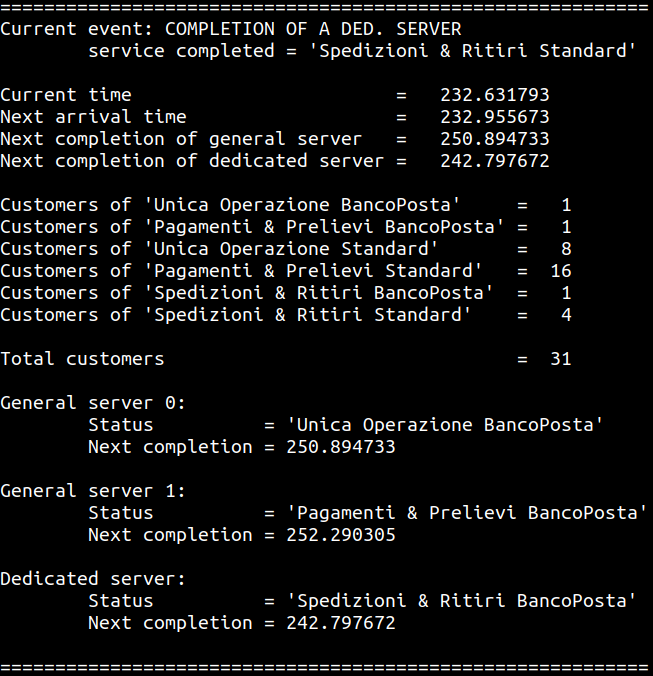
\includegraphics[width=\textwidth]{screenshots/original/ded_server_priority_sched}
\caption{Schedulazione sul server dedicato}    
\label{fig:verifica-1b}
\end{subfigure}


\vskip\baselineskip

\begin{subfigure}[b]{0.475\textwidth}   
\centering 
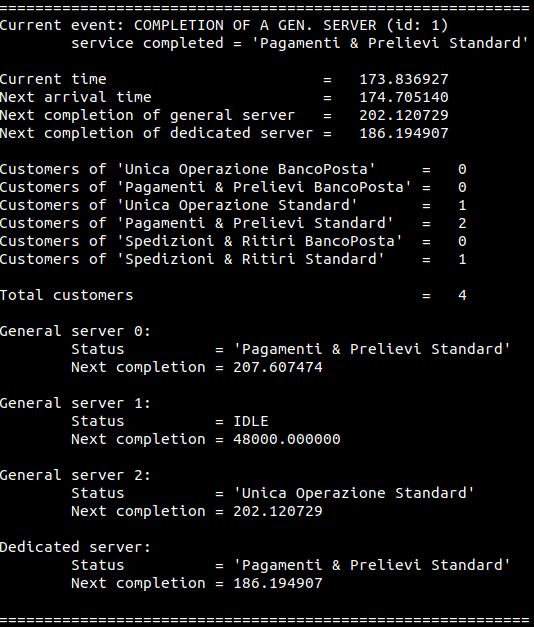
\includegraphics[width=\textwidth]{screenshots/original/gen_servers_no_SR}
\caption{I server generali non processano \sr{}}   
\label{fig:verifica-1c}
\end{subfigure}
\hfill
\begin{subfigure}[b]{0.475\textwidth}   
\centering 
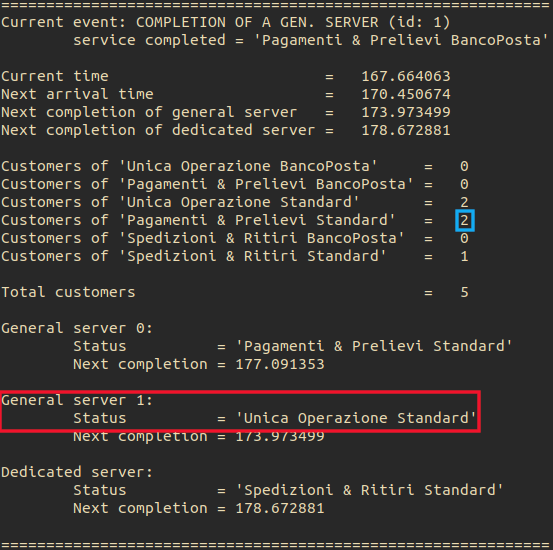
\includegraphics[width=\textwidth]{screenshots/original/gen_servers_priority_sched}
\caption{Schedulazione su un server generale}    
\label{fig:verifica-1d}
\end{subfigure}
\caption{Screenshots della simulazione per la fase di verifica}
\label{fig:verifica-1}
\end{figure}

I controlli di consistenza effettuati sono di seguito analizzati:
\begin{itemize}
\item In assenza di ticket di tipo \sr{} da processare, il server dedicato si comporta come se fosse generale, ovvero elaborando, se presenti, richieste \uo{} o \pp{} (fig. \ref{fig:verifica-1a}).
\item In presenza di ticket di tipo \sr{} da processare, il server dedicato ignora le altre code e processa tali richieste dando priorità ai titolari di conto \textsl{BancoPosta} (fig. \ref{fig:verifica-1b}).
\item Pur essendo \texttt{IDLE}, i server generali non possono processare richieste di tipo \sr{} (fig. \ref{fig:verifica-1c}).
\item Un server è \texttt{IDLE} se e solo se non sono presenti richieste pendenti che è in grado di processare (fig. \ref{fig:verifica-1c}).
\item In fase di schedulazione, i server generali processano le richieste secondo l'ordine di priorità specificato nei modelli precedenti (fig. \ref{fig:verifica-1d}).
\end{itemize}

In particolare, gli screenshot riportati in figura \ref{fig:verifica-1}, e sopra più volte referenziati, sono stati tutti quanti realizzati fissando come seed iniziale \texttt{9}.